%==========================================================================================================================
% (c) Vojtěch Kulička, 2010

\chapter{Introduction}
Human is a social creature and likes to chat, share feelings and ideas. At first we managed to do so by making simple sounds. Those sounds later on developed into words. Then much later the human race started to feel the need to record what we were thinking. We made up symbols and started to write. As the society grew and spread, we wanted to communicate with people from other tribes and villages. At first we would travel and use spoken words, but as the distances grew we figured we can have our thoughts delivered in writing. Mail was born. In 1844 telegraph was invented by Samuel Morse followed by telepthone in 1874 by Alexander Graham Bell. And finally in 1969 the Internet was created. All of these inventions aimed to provide means of communication to satisfy the needs of the evolving society.  

In the early days of the Internet email was the main means of communication. And just like regular mail people would have their electronic mailboxes to which the emails were delivered. Email was a huge step forward for it provided a way to almost instantly deliver text from one place to another regardless of the distance for free. The main disadvantage of email is that people had to check their mailboxes read new mail and then reply. It is just neither fast nor convenient enough for team cooperation when team members are far apart. For those and other purposes like chatting Instant Messenger programs were introduced.    

An IM program offers realtime communication between two people via text messages that are delivered from one user to another instantly. Instant messangers became very popular and started adding on features like multiuser chat, various games and most importantly VoIP(Voice over IP) support. VoIP capable IM like skype have become extremely popular at first for making it possible for people to call each other for free over the internet. Later video conferencing capability was added, so you could talk and see you colleague at the same time. One more thing comes in extremely handy when working in a team - a whiteboard.

At this time there is no usable IM providing VoIP and shared whiteboard for GNU/Linux. This thesis aims to add VoIP support to an existing XMPP client with shared board called Makneto. Makneto was created by Jaroslav Řezník as a master's thesis in 2008. At this point it is using iris library for XMPP communication. The shared board data is also transferred over XMPP. One of the goals of this thesis is to port Makneto to telepathy, which is now a very reliable and robust library for communication for numerous protocols.  

The following chapter gives a detailed description of the current version of program Makneto. We will find out about it's architecture, strengths and weaknesses. 

Chapter number three focuses on XMPP/Jabber communication protocol. It talks about it's features and limitations. 

Chapter three is about Telepathy communiation framework, how it works, what it consists of. There is also a description of a IM client application Empathy based on Telepathy. 

Current audio and video streaming protocols are listed and discussed in chapter five. Based on this chapter a suitable protocol is chosen for the implementation.

Finally the implementantion of VoIP into Makneto is in chapter six.  

% =========================================================================================================================
% =========================================================================================================================

\chapter{Makneto}
Makneto is an instant messenger with a shared board capability. It was written by Jaroslav Řezník as his master's thesis in 2008. Makneto is written in C++ using Qt version 4 and KDE 4 libraries. Qt is a application framework written in C++. Qt extends C++ and instead of callback function uses a concept of signals and slots, which is as opposed to callback functions type-safe. It runs on all major computer platforms like GNU Linux, Microsoft Windows and Mac OS X. Moreso it is supported by mobile device platforms such as Symbian and Microsoft Windows Mobile. There is also a port to Google Android called Lighthouse. Qt was developed by company named Trolltech and was available under two licenses. First was a commercial license allowing companies to write proprietory applications for a fee. Second was GNU General Public License, which was of course free. Thanks to the commercial license the Qt documentation is one of the best among any software available under GNU GPL. In june 2008 Troltech was acquired by Nokia. Nokia decided to make the source code available so that anyone could contribute. In January 2009 with the release of Qt 4.5 another licensing option was added - Lesser General Public License.\cite{wikiQt}\cite{Qt}

Besides Qt Makneto utilizes functionality provide by KDE 4\cite{KDE} libraries, which makes Makneto unable to run on a different operating system than GNU Linux. KDE is a desktop environment created by Matthias Ettricht in 1996 for he felt the need for a good quality window manager for Linux. KDE is currently in version 4, which brought great features. There is a new desktop called Plasma, which allows users to display widgets called plasmoids directly on the desktop. That allows users to have a TODO list, calendar, translator, weather forecast, system monitor and much more right in front of them on their desktops without having launch any of those to get the information they need. It makes users' work eesier and more efficient. KDE and GNOME are the most common window manager in Linux. GNOME offers stable useful environment and is influenced mostly by large businesses using it. KDE is more flexible and works more with the look and feel.

Makneto communicates using XMPP/Jabber protocol implemented in Qt-based C++ library called Iris. All of the Iris is primarily used by Psi instant messenger. It's development is still quite active and it supports all of Jabber's key features. Iris' downside is very poor documentation. It's wiki is very brief and all to all gives one example. The only way to find out how it works is browsing through Psi code.\cite{irisWiki}

Makneto's shared whiteboard is based an official extension of XMPP SVGWB by Joonas Govenius\cite{SVGWB}. SVGWB is implemented in Psi and Makneto utilizes their code. SVGWB defines all the necessary actions like whiteboard session initianion including invitation and mainly how to send and receive information about the grahical objects using XMPP text messages. The actual graphical object representation is defined by SVG\cite{SVG}(Scalable Vector Graphics) by W3C. SVG describes graphics objects using vectors in XML format. Makneto uses just a subset of SVG called SVG Tiny\cite{SVGtiny} as it does not need all of the features of SVG. Tiny SVG describes two-dimensional vector graphics and raster graphics and multimedia. To sum up Makneto's whiteboard features, it allows you to draw lines, rectangles, elipses, circles, sketch using a paintbrush and input images in jpg and png formats. Graphical objects are resizeable, can be rotaded and copied.  

Makneto runs in one window (see figure \ref{fig:makneto}). User's contact list is on a panel on the left hand side. The whiteboard and chat session are initiated through the contact list. Makneto handles more session at once each in a separate tab. Using the application is very comfortable although it from dies time to time.

%TODO - pic of makneto

% =========================================================================================================================
% =========================================================================================================================

\chapter{XMPP}
%Extensible Messaging and Presence Protocol
%XML based
%IETF standard
%

% =========================================================================================================================
% =========================================================================================================================

\chapter{Telepathy}
Telepathy\cite{telepathy} is a modular communications framework for building real-time communication applications. It supports numerous communication protocols as plugable backends e.g XMPP/Jabber(telepathy-gabble), SIP(telepathy-sofiasip), MSN(telepathy-butterfly) etc. Each of telepathy's components runs in a separate process as desktop service and communicates via D-Bus. The components are shared by telepathy clients. For example if there are two clients using XMPP they both use the same instance of telepathy-gabble. To get a better idea of how this concept works take a look at figure ~\ref{fig:telepathyArchitecture}.\cite{TPWiki} 

\begin{figure}[ht]
\begin{center}
	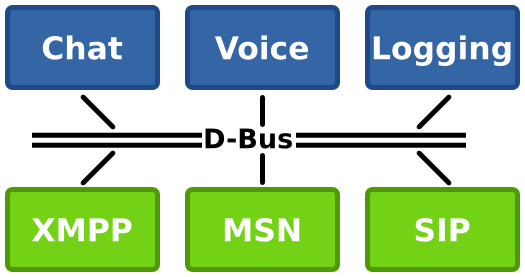
\includegraphics[width=10cm]{fig/telepathy-architecture-overview.png}
	\caption{Telepathy architecture\cite{TPWiki}}
	\label{fig:telepathyArchitecture}
\end{center}
\end{figure}


There are several features making telepathy very useful as a communications framework.

\begin{itemize}

	\item {\bf Robustness} - all the components are independent. If one crashes, others will not be affected

	\item {\bf Ease of development} - the components can be replaced without having to stop the service 

	\item {\bf Language independence} - since telepathy components use D-Bus for communication among themselves, any language that has D-Bus binding might be used to write them

	\item {\bf Desktop independence} - D-Bus is present in both main Linux window managers GNOME and KDE, so the same telepathy components could be backend for appropriate frontends.

	\item {\bf Code reuse} - the client applications do not have to worry about protocol specifics, which are handled by Telepathy. The client can use more protocols by making no or small alterations to the code.

	\item {\bf Connection reuse} - more than one Telepathy client can use the same connection simultaneously:
\end{itemize}

\section{Telepathy basic terminology}
Telepathy is a very powerful framework and as such it is also complicated. To successfuly write programs using Telepathy we need to know what telepathy consists of and what it is based on. 

\subsection*{D-Bus}
D-Bus is a kind of inter-process communication. It allows two applications running in different processes, written in different programming language communicate. More so these applications may communicate directly, without having to go through message bus daemon. There two types of D-Bus. First is a system bus used for events such as ``USB device disconnected'' or ``printer out of paper.'' Second type is per-user-login-session bus, which is used by user applications. D-Bus low level API is represented by libdbus and it requires XML parser(libxml or expat) to work. Higher level language bindings such as Qt, GLib, Java etc. are built on top of libdbus and offer more convenient way of using D-Bus, although they add more dependencies.\cite{dbus}\cite{TPWiki} 

Each process that wants to communicate over D-Bus will need to use most the following depending on it's nature: 
\begin{itemize}
	\item {\bf Unique name} - is an unique id(e.g. 2.1) assigned by D-Bus daemon to the client application. Unique name is similar to a public IP address.
	\item {\bf Wellknown name} - is similar to a DNS name. If a process wants to make a service available to other processes it requsets a wellknown name. If another process wants to access the service it uses the wellknown name to do so. Wellknown name might look like this: org.freedesktop.Telepathy.ChannelDispatcher.    
	\item {\bf Object path} - is a path to an object that is exported by process running a service.
	\item {\bf Interface} - is a way of requesting a service using signals or methods. Each D-Bus client must register at least one interface and each interface provides at least one method or signal. Every interface needs to have to name like a wellknown name.  
	\item {\bf Method} - is impleneted in the object specified by object path and exposed in the interface for that object for other processes to use. 
	\item {\bf Signal} - is a D-Bus signal client process can connect to it's callback function. If a signal is invoked the callbacked function is called.
	\item {\bf Property} - is used for exposing D-Bus object's properties. To do so the objet must implement org.freedesktop.DBus.Properties interface.
\end{itemize}

The following figure \ref{fig:dbusArchitectureNames} shows an example of two programs connected to D-Bus to be able to communicate with each other. Program B provides a service called org.freedesktop.foo.Bar(wellknown name) and it's id is 1.3. Program A does not provide any service and thus does not need any wellknown name. It just needs an id(1.2) to use other programs' services.\cite{TPWiki}

\begin{figure}[ht]
\begin{center}
	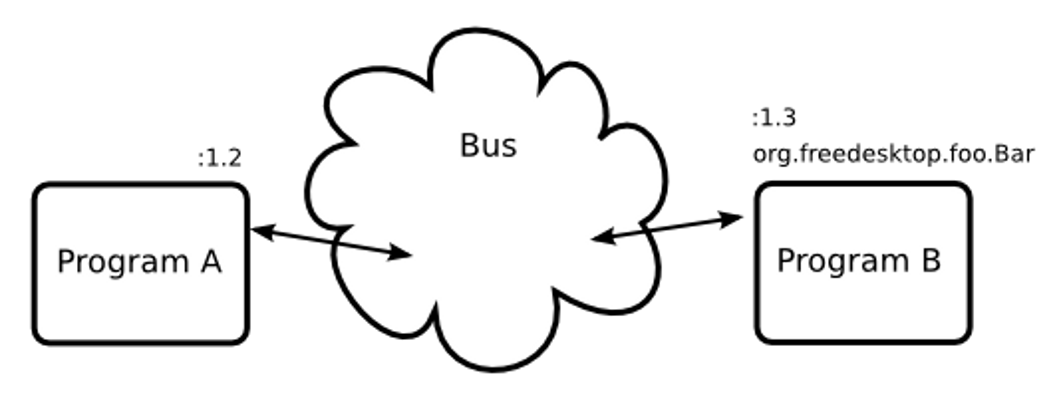
\includegraphics[width=11cm]{fig/dbus-architecture-names.png}
	\caption{D-Bus id and wellknown name example\cite{TPWiki}}
	\label{fig:dbusArchitectureNames}
\end{center}
\end{figure}


The figure \ref{fig:dbusArchitecture} shows an overview of all of the terms described above in a simple diagram.

\begin{figure}[ht]
\begin{center}
	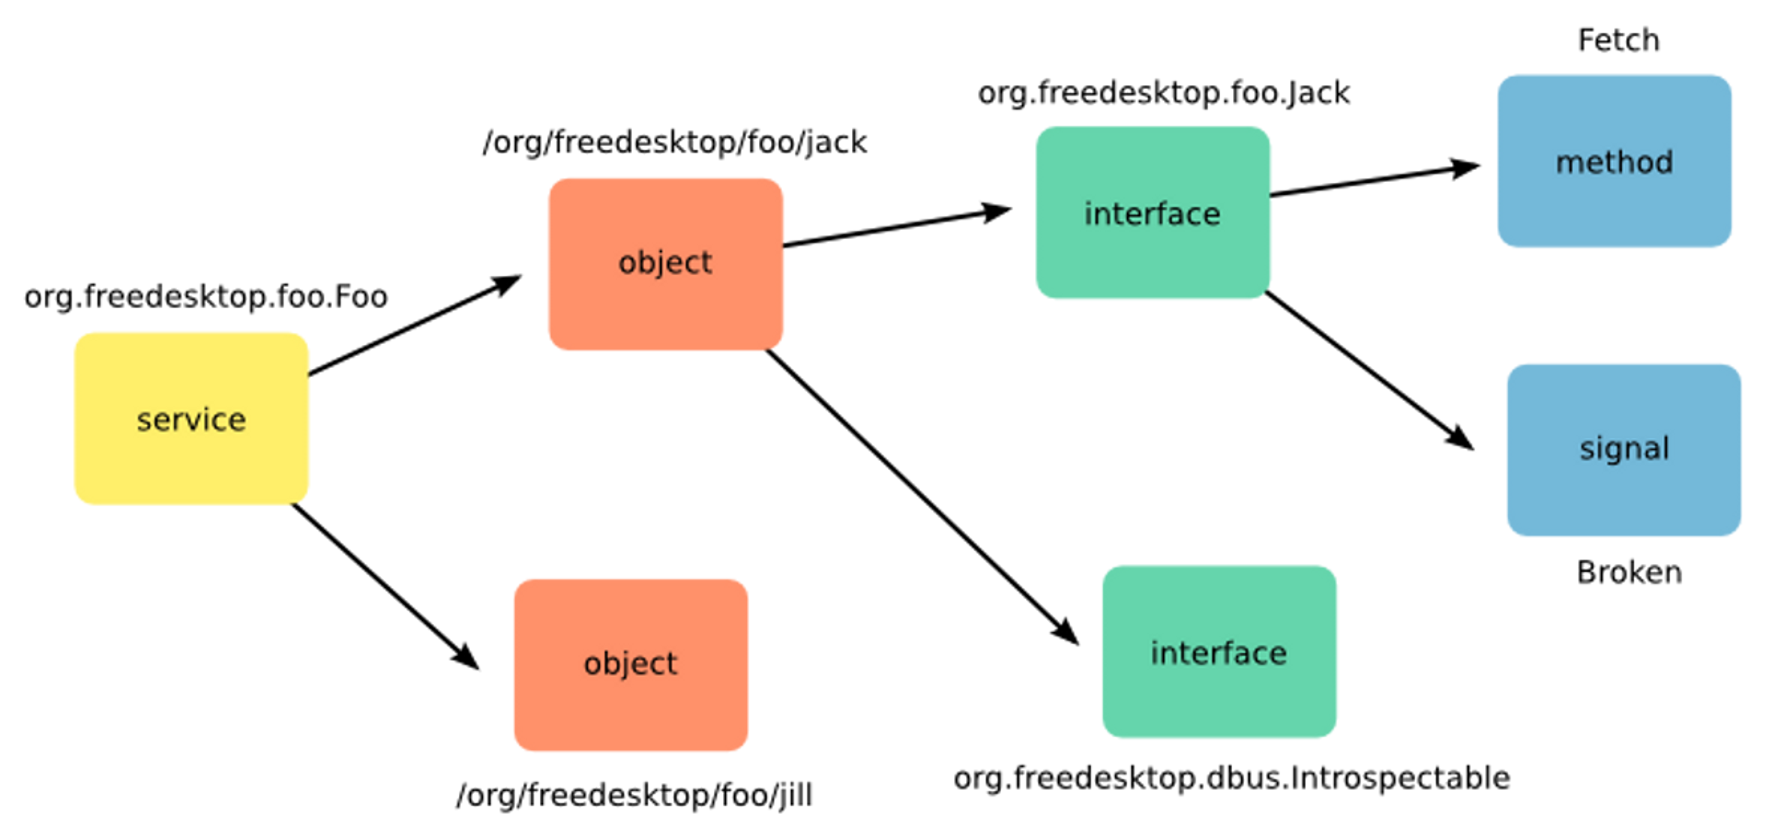
\includegraphics[width=15cm]{fig/dbus-architecture-overview.png}
	\caption{D-Bus architecture\cite{TPWiki}}
	\label{fig:dbusArchitecture}
\end{center}
\end{figure}

D-Bus is a key component of Telepathy framework. Telepathy supports many protocols all of which might provide different capabilites. For example IRC does not support avatars while XMPP does. Eventhough avatar feature is supported by XMPP protocol it might not be supported by the server we are connected to or by the opposite client in case of peer-to-peer connection. The available features are exposed by D-Bus Properties Interface. That is an easy way of determining the protocol, server or client capabilities.\cite{dbus}

\subsection*{Mission Control}
Mission Control is a Telepathy component that implements Account Manager and Channel Dispather and it's primary purpose is to encapsulate those two.\cite{TPWiki}

\subsection*{Account Manager}
Account Manager is responsible for handling accounts(e.g. XMPP, ICQ, MSN etc.). It is accessible by well-known name on D-Bus - org.freedesktop.Telepathy.AccountManager. A client application first creates an account using the CreateAccount() method, supplying it with ConnectionManager, protocol and display name. Account Manager creates and then as long as the account is active maintains Connection to that account. To create a Connection a Connection Manager is called. An account may be valid or invalid. Valid accounts may establish a Connection, whereas invalid can't. The list of valid and invalid accounts is accessible via ValidAccounts and InvalidAccounts properties respectively.\cite{TPWiki} 

\subsection*{Account}
When the Account Manager's CreateAccount() is called it returns an Account object. Account object registers with D-Bus and has an object path /org/freedesktop/Telepathy/Account/CM/PROTOCOL/ACCDN. CM stands for Connection Manager(e.g. gabble, salut, butterly etc.), PROTOCOL is substitution for a protocol name and ACCDN is Account Display Name. The Account object implements org.freedesktop.Telepathy.Account interface. Features supported by this interface depend on the protocol used and the server-side software. The Account settings are done via org.freedesktop.Telepathy.Properties interface. All available attributes can be obtained by calling the GetAll() method provided by the Properties Interface. The GetAll() method is very convenient for it returns all the propeties at once in signle D-Bus call. Similarly there is a method for setting all properties at once - Account interface's UpdateParameters() method. The following tables lists all properties of the Account object available. Table \ref{table:configureableProperties} shows properties that can be configured and table \ref{table:nonConfigurableProperties} shows properties just for reading. Some features are available via specified interface, e.g. avatar. Avatar used to be a property, but now it has it's own interface. The Interfaces property of the account lists all interfaces of additional features.\cite{TPWiki}

\subsection*{Connection Manager}
Connection Manager supplies Account Manager with Connections. It is not directly used by the client program. Account Manager requests connection for active accounts.

Connection Manager is a protocol-dependent Telepathy component. Different protocols need different Connection Managers. For example if the client application wants to communicate using XMPP/Jabber it has to use Telepathy-gabble and for MSN Telepathy-butterfly is required. Some Connection Managers can communicate via more than one protocol, for example Telepathy-haze. To see what protocols are supported there is ListProtocols() method implemented by the Connection Manager.\cite{TPWiki}

\subsection*{Connection}
Connection represents an active protocol session. It is associated with an Account and is created by Connection Manager based on a request of the Account Manager. Connection implements org.freedesktop.Telepathy.Connection interface and additional interfaces depending on the protocol. List additional interfaces available can be retrieved by checking the Interfaces property. The most common interfaces are listed below\cite{TPWiki}:

\begin{itemize}

	\item {\bf Contacts} - used to get as much information about a contact as asked in one D-Bus call.

	\item {\bf Aliasing} - serves for setting aliases for contacts and checking if the contacts have changed their alias themselves. 

	\item {\bf Avatars} - interface to one of the most popular protocol features. Allows users to set their avatars and retrieve other users' avatars.

	\item {\bf ContactCapabilities} - retrieves capabilities of contacts' Clients to see what features they support. Checks for example for VoIP or file transfer support.

	\item {\bf Location} - lets user publish his or her current location as well as find out his or her contacts' whereabouts. 

\end{itemize}


\subsection*{Channel Dispatcher}
This component handles Channels incoming from active Connections of valid Accounts. Channel Dispatcher monitors available or activatable Telepathy Clients through D-Bus. Clients register with user's session D-Bus and provide a CLIENT\_NAME.client file. Both of those serve as a way to publish Client's properties including a channel filter. The Channel Dispatcher based on these properties knows what kind of a client it is and what type of channels it is interested in (channel filter). If the Client is running then the properties are acquired via the Client interface. If the client is not running and is activatable then the .client file is used by Channel Dispatcher to pre-look up the properties and if they match the incoming Channel, the Client is activate.So providing the .client file only makes sense for activatable Clients.  

When a Channel comes in from one of the Connections Channel Dispatcher notifies appropriate Clients. There are three kinds of clients - Observer, Approver and Handler(see \ref{subsect:tpClient}). The Channel is dispatched to all Observers and all Approvers with a matching channel filter. The Approvers choose Handler to handle the Channel. Should the Client fail, Channel Dispatcher may recover from such error and look for another Handler.\cite{TPWiki}  


\subsection*{Channel}
Channel allows the local client to exchange various kind of data with a remote server. It is associated with a Connection and always implements at least two interfaces. The first is org.freedesktop.Telepathy.Channel and the second depends on the Channel type. Channels for text messaging will be of type Text and will implement org.freedesktop.Telepathy.ChannelType.Text interface. The following list shows most common types of Channels\cite{TPWiki}:

\begin{itemize}

	\item {\bf ContactList} - used to get information of contacts in user's contact list.

	\item {\bf Text} - designed for exhanging text messages. 

	\item {\bf Call} - used for VoIP and video calls. 

	\item {\bf FileTransfer} - Channel for sending and receiving files.

	\item {\bf ContactSearch} - is used when a user wants to find a contact on a server.

\end{itemize}

Channels are created using two methods - CreateChannel() and EnsureChannel(). These methods are implemented by both Channel Dispatcher and Connection. When calling either of those methods on Channel Dispatcher the resulting Channel will go through the procedure of looking for handler as described above. When using directly the connection the calling application must handle the Channel itself as the Channel Dispatcher will not interfere. It is also possible to supply the Channel Dispatcher with a preferred handler and thus achieve the same effect. It is better to use the Channel Dispatcher for if the client should fail it may dispatch the Channel to another handler.\cite{TPWiki}

Both CreateChannel() and EnsureChannel() methods provide a Channel. The difference between the two is that CreateChannel() creates actual new Channel whereas EnsureChannel() will attemp to reuse an existing Channel with the same properties. If there is no Channel to be reused or it is being used by a different application than it creates a new Channel, just like CreateChannel(). Typicaly CreateChannel() is used for FileTransfer and ContactSearch and EnsureChannel() for Text, StreamedMedia and ContactLists Channels.\cite{TPWiki} 

\subsection*{Client}\label{subsect:tpClient}
Client is an application that wants to use Telepathy. It needs to register a well-known name in org.freedesktop.Telepathy.Client namespace, e.g. Empathy registers org.freedesktop.Telepathy.Client.Empathy. Then it provides a .client file where purpose of which is described above. Telepathy defines three types of clients - Observer, Approver and Handler. All of these need to provide appropriate channel filter, e.g. Oberver provides ObserverChannelFilter. Based on the published filter the Channel Dispatcher dispatches an incoming Channel to the Client or not.\cite{TPWiki}  

Observers are called upon a creation of a new Channel. They monitor Channels and provide the acquired information to user. The observers have different functions based on the type of observed Channel, e.g. Text Channel observer might serve as a logger and FileTransfer observer as a file transfer progress monitor. Observer is must not interfere except for when the user interaction like hitting the cancel button in a file transfer progress window.\cite{TPWiki}     

Approver is a Telepathy Client that is supposed to accept the incoming Channel and decide, which Handler it is dispatched to. The Channel Dispatcher provides Approvers with a list of possible Handlers. Approver notifies the user of a new Channel and lets him or her decide whether to accept or reject it. Similarly the user is allowed to choose which Handler will handle the Channel. Handler might also be chosen by the Approver itself. Approver does not call methods just like the Observer. Calling methods is up to the Handlers. For example if there is an incoming file transfer the Approves lets user decide whether to accept it or not, but the AcceptFile method will be called by the chosen Handler.\cite{TPWiki}  

The last client is Handler. Handler does all the interaction with the Channel. A typical example of a Handler is chat-window. It displays messages and allows the user to send text messages back.\cite{TPWiki}  

%\subsection*{Handle}
%Telepathy handles represent objects like contact, roster, chatroom etc. It is a number, assigned by Connection the object is related to, that identifies the object. In addition to the numeric id handles also have a string id(e.g. chatroom could have a string id makneto@jabber-discussion.com). Depending on the protocol resource the handle represents it is of an apropriate type(Handle\_type property). Handles with different types may have the same numeric id. When comparing handles it should be always done by comparing the numeric id's, assuming we are comparing handles of the same type.\cite{TPWiki} 


\begin{figure}[ht]
	\begin{center}
	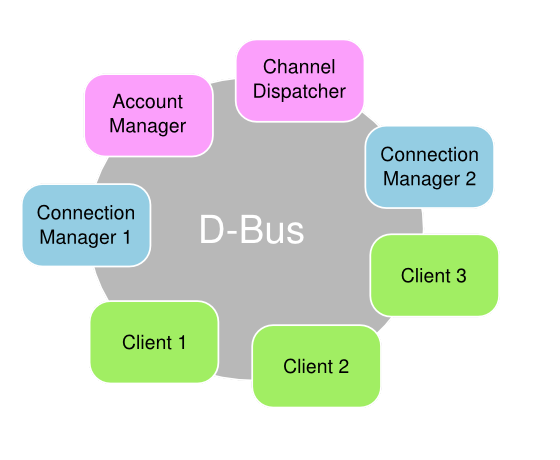
\includegraphics[width=10cm]{fig/telepathy-components-dbus.png}
	\caption{Telepathy components registered with user session D-Bus.\cite{TPWiki}}
	\label{fig:telepathyComponentsDbus}
\end{center}
\end{figure}

The figure \ref{fig:telepathyComponentsDbus}

%\section{Telepathy language bindings}
%Telepathy clients may be written using language bindings. These bindings must provide D-Bus API. 
%Telepathy-glib, Telepathy-python
%Telepathy-qt4

\section{Empathy}
Empathy is a multiprotocol instant messaging application based on Telepathy. In the terms described above Empathy is a Telepathy client. It is written in python using Telepathy-python bindings. Empathy registers a well-known name with D-Bus and communicates with Telepathy components to provide the communication services. Empathy supports text messaging, file transfer, voice and video calls over various protocols. Supported protocol include Google Talk, XMPP/Jabber, MSN, IRC, AIM Facebook, Yahoo!, Gau Gadu, and ICQ. For some of those protocols like Google Talk and XMPP voice and video calls implemented. The suppport of the protocols depend on Telepathy Connection managers installed. Additional functionality includes sharing users' whereabouts among themselves, automatic reconnection when internet connection is reestablished and automatic changes of presence to away and extended away.\cite{empathyGnome}

The current stable version of Empathy is 2.32.2 and it is a default communication application in GNOME releases since version 2.24 instead of Pidgin. Empathy also replaced Ekiga - program for voice calls and video-call. It became an ultimate free communication tool. Empathy's GUI is takes after Gossip, which is an older IM application for GNOME. 

% =========================================================================================================================
% =========================================================================================================================

\chapter{Existing solutions with whiteboard and VoIP}

%\section{SIP}
%\section{RTP}

There is a number of existing communication applications offering voice calls and shared whiteboard. Some more popular, more advanced, more user-friendly, offering more features or better support than others. Some of those program support video call and some even conference calls. We shall go over the existing solutions that implement both shared whiteboard and voice calls. Among the described are Skype\cite{skype}, Windows Live Messenger\cite{WindowsLiveMessenger}, Brosix\cite{brosix}, Yahoo! Messenger\cite{yahoo} and AIM\cite{AIM}.

\section*{skype}
Skype is the most popular and most used common VoIP application of all. It is available for all major computer platforms (Microsoft Widnows, Mac OS X and GNU Linux) as well as mobile platforms like Android and even Apple's iOS. Although skype is available for Linux it is not well supported. The latest version of skype for Linux is 2.1.0.81 Beta while skype for Windows is of version 5.1. Finally skype is built-in on more and more TVs.

Skype communicates using Skype protocol, which is proprietory. Recently much effort is being put in reverse engineering the skype protocol. The motivation for this is simple. Skype is used by tens of millions of users every day, but the support for Linux is at this point almost nonexisting. Linux users have had enough and plan to create an open source client capable of communicating with skype. The wikipedia skype protocol page\cite{wikipediaSkypeProtocol} is filling up with details. While most of IM programs utilize client-server communication scheme, skype uses peer-to-peer model. The skype network consists of nodes, supernodes and login servers(see figure\ref{fig:skypeArchitecture}). Nodes are clients. Each client keeps addresses of a number of supernodes. Supernodes are clients with good-enough bandwith and public IP address. Supernodes forward traffic to clients behind NAT, PAT or restrictive filters. This decentralized architecture seems to be working well although there was an outage on December 22nd 2010. Skype officials claim it was due to lack of supernodes\cite{skypeOutage}.  

Features of skype include calling landlines and cell phones and sending text messageses and vice versa - SkypeOut and SkypeIn. The feature list continues with voice and video calls, multi-user chat, conference calls, voice mail and screen sharing. The newest and long expected feature of video conference was introduced in may of 2010 in skype 5.0. 

Though closed program, skype provides an API for developers who want to create extensions called skype extras. Skype extras include a wide range of utilities that might be plugged into skype. The extras uSeeToo, TalkAndWrite, WhiteBoardMeeting and Sketch Pad all provide shared whiteboard each in their own way.    

% TCP for signaling and TCP and UDP for transport
% wideband codec 
% 

\begin{figure}[ht]
	\begin{center}
	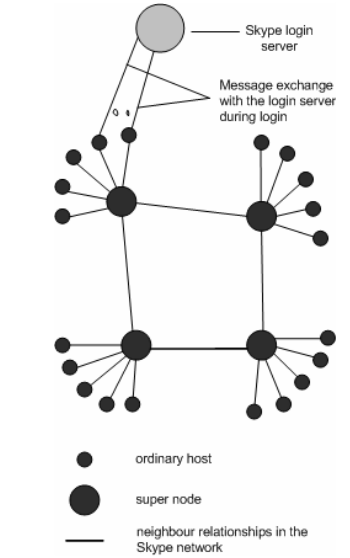
\includegraphics[width=10cm]{fig/skype-architecture.png}
	\caption{Telepathy components registered with user session D-Bus.\cite{skypeAnalyzed}}
	\label{fig:skypeArchitecture}
\end{center}
\end{figure}

\section*{Windows Live Messenger}
Windows Live Messenger was first released in July 1999 as MSN Messenger and offered just text messaging with users of AOL Instant Messenger\cite{AIM}. Due to AOL's constant effort to block Microsoft from it's network Microsoft gave in and removed the feature. Since then MSN Messenger could only connect to MSN Messenger Service. In 2001 with the release of Windows XP, MSN Messenger 4.6 came out with voice call support. The last version of MSN Messenger, version 7.5, featured video calls. Windows Live Messenger 8.0 was released in june 2006 and that was the end of the name MSN Messenger.   

Windows Live Messenger utilizes client-server model and communicates using Microsoft Notification protocol over TCP. The first 7 versions of MSNP were disclosed to public, but since version 8 the details have been kept a secret. MSNP does not use encryption so eventhough MSNP's description was not published it was not hard to put it together using packet sniffers.

The live Messenger is available for Windows, Mac OS X and recently was integrated into Microsoft's game console Xbox 360. It features social network integration, offline messaging, games and applications, voice and video calls and standard IM features. An interesting feature is Multiple points of presence allowing user to be connected on two devices. Shared whiteboard is available as an extra application and is not capable of multi-user session.   

\section*{Brosix}
An award winning application first released in 2006. Brosix features voice and video chat and multi-user chat, basic IM functions and couple advanced functions. Brosix's whiteboard is an Microsoft Paint like window shared among the participants and won Best IM Feature 2009 award from about.com. Next great feature allows users share screen, including mouse and keyboard much like VNC. Finally Brosix implements co-browsing where users share a browser window. 

Brosix is available for Windows, Max OS X and GNU Linux in commercial and personal(free) version. There is little known about used technologies and it is almost impossbile to reverse-engineer using packet sniffers as Brosix uses 256 bit AES encryption.

\section*{Yahoo! Messenger}
Yahoo! Messenger is just like all of the above a closed program though some information has leaked\cite{wikipediaYahoo}. Yahoo! Messenger protocol(YMSG) uses TCP on port 5050 or a different one if default is unavailable. To get to clients behind firewall HTTP is utilized. Video and voice supposedly use SIP and H.323.

Besides the standard set of IM functions Yahoo! Messenger can call PSTN, send SMS and handle voice conference. Whiteboard feature is called Scribbler and is plugin. Linux is missing in the list of supported platforms while Windows and Mac OS X are not.

\section*{AOL Instant Messenger}
AIM is yet another IM with proprietory communication protocol. Though AIM is a bit of an exception for it supports two protocols. First is just for simple text messaging called TOC and has been disclosed to public. Second protocol that supports all of the advanced features is being kept a secret.

AOL's messenger is available for Windows and Mac OS X and features voice and video calls as well as whiteboarding. Whiteboard is available as a plugin for AIM called IM Whiteboard. 

% =========================================================================================================================
% =========================================================================================================================

%\chapter{Implementation}

% =========================================================================================================================
% =========================================================================================================================

\chapter{Conclusion}
Závěrečná kapitola obsahuje zhodnocení dosažených výsledků se zvlášť vyznačeným vlastním přínosem studenta. Povinně se zde objeví i zhodnocení z pohledu dalšího vývoje projektu, student uvede náměty vycházející ze zkušeností s řešeným projektem a uvede rovněž návaznosti na právě dokončené projekty.

